\section{Aula 18 de Novembro de 2019}
\label{2019_11_18}

\subsection{Introdução}

Observe a ilustração abaixo, onde cada ponto colorido foi sorteado uniformemente dentro do quadrado de lado $2$. Qual é a probabilidade de um ponto qualquer cair dentro do círculo unitário, ou seja, ser vemelho? Mais formalmente, dado um conjunto de $m$ pontos $u_1, \dots, u_m \in_U [-1,1]^2$, quanto vale $\PP(u \in \text{disco unitário})$?

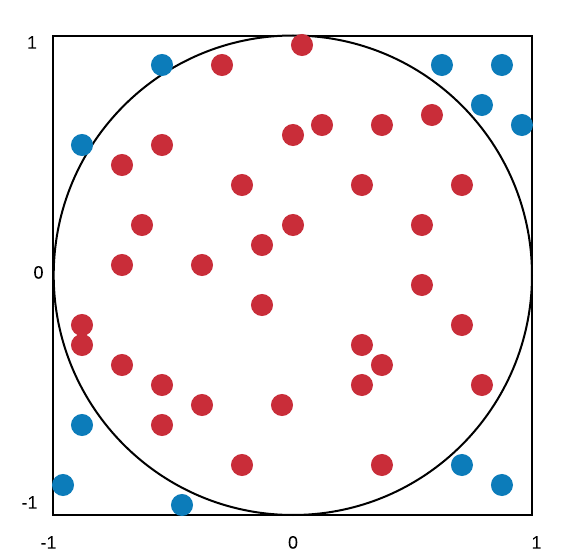
\includegraphics[width=0.25\textwidth]{aulas/11_18/PiBoard.png}

Calcular essa probabilidade é simples: $\PP(u \in \text{disco unitário}) = {\text{área do círculo unitário} \over \text{área do quadrado } [-1,1]^2} = {\pi \over 4}$. Partindo deste ponto, considere agora a variável indicadora

$$
z_i = \mathbbm{1}\{u_i \in \text{disco unitário}\} = 
\begin{cases}
    1, & \text{se } u_i \in \text{disco unitário} \\
    0, & \text{caso contrário},
\end{cases}
$$ e seu somatório (para todos os $m$ sorteios) $z = \sum_{i = 1}^m z_i$.

É fácil ver que, dadas as definições acima, $\PP(z_i) = {\pi \over 4}$ e $\EE(z_i) = {\pi \over 4}$. Ademais, $\EE(z) = \EE\big(\sum_{i = 1}^m z_i\big) = \sum_{i = 1}^m E(z_i) = m {\pi \over 4}$. Com estes fatos, determina-se uma estimativa para $\pi$: $z’ = {4 \over m} z$. Experimentos como este, de amostragem repetitiva capazes de obter aproximações, são exemplos do método de Monte Carlo.

\subsection{$(\varepsilon, \delta)$-aproximação}

Considerando ainda os objetos definidos acima, $z$ tem distribuição $\mathrm{Bi}\big(m, {\pi \over 4}\big)$ e assim é fortemente concentrado em torno da média, ou seja, a probabilidade de $z'$ estar entre $(1-\varepsilon)\pi$ e $(1+\varepsilon)\pi$ é $\geq 1- \delta$. De fato, se $\varepsilon \leq {3 \over 2}$, então
\begin{align*}
  &P( | z’ - \pi | \geq \varepsilon \pi) \\
      &= P\Big(\Big| {4 \over m}z - \pi \Big| \geq \varepsilon \pi\Big) \\
      &= P\Big(\Big| z - {m \over 4}\pi \Big| \geq {m \over 4} \varepsilon \pi\Big) \\
      &\leq 2e^{- {1 \over 3} \varepsilon^2\big({m \over 4}\pi\big)}.
\end{align*}

Logo, se $m \geq {12 \over \varepsilon^2 \pi} \log \big({2 \over \delta}\big)$, então $P( | z’ - \pi | \geq \varepsilon \pi) \leq \delta$. Se realmente $|z’-\pi| \leq \varepsilon \pi$, então $(1-\varepsilon)\pi \leq z’ \leq (1+\varepsilon)\pi$ e assim pode-se concluir que, se $\varepsilon \leq {1 \over 2}$.
$$(1-\varepsilon)z’ \leq {z’ \over 1 + \varepsilon} \leq \pi \leq {z’ \over 1 - \varepsilon} \leq z’(1+2\varepsilon) \text{, ou seja, } (1-\varepsilon)z’ \leq \pi \leq (1+2\varepsilon)z’.$$

\begin{definicao}
Dizemos que o algoritmo $\mathscr{A}$ fornece uma $(\varepsilon, \delta)$-aproximação de $V$ se $\mathscr{A}$ tem como saída um vetor $\mathbf{x}$ tal que $P(|x - V| \geq \varepsilon V) \leq \delta$.
\end{definicao}

Como vimos anteriormente, se $m \geq {12 \over \varepsilon^2 \pi} \log \big({2 \over \delta}\big)$, então $m$ amostras $u_i \in_U [-1, 1]^2$ fornecem uma $(\varepsilon, \delta)$-aproximação para $\pi$.

\begin{teorema}
\label{teorema:edaproximacao}
Sejam $z_1, \dots, z_m$ variáveis indicadoras independentes com $\EE(z_i) = \mu$ para todo $i$. Então, se $m \geq {3 \over \varepsilon^2 \mu} \log \big({2 \over \delta}\big)$, $\PP\big(\big|{1\over m} \sum_{i = 1}^m z_i - \mu\big| \geq \varepsilon \mu\big) \leq \delta$. Isto é, $m$ amostras fornecem uma $(\varepsilon, \delta)$-aproximação de $\mu$.
\end{teorema}

De forma mais geral, temos uma função $V: x \mapsto V(x)$. Dois exemplos:
\begin{enumerate}
\item Grafo $G \mapsto V(G)$, onde $V(G)$ é o número de emparelhamentos perfeitos em $G$,
\item Fórmula booleana $\varphi \mapsto V(\varphi)$, onde $V(\varphi)$ é o número de valorações das variáveis de $\varphi$ para tornar $\varphi$ verdadeira.
\end{enumerate}

Acredita-se que certos problemas de contagem são difíceis (em termos da teoria da complexidade) a menos que P = NP. É o caso dos exemplos acima.

\subsection{FPRAS}

\begin{definicao}
Dizemos que um algoritmo $\mathscr{A}$ é um FPRAS (fully polynomial randomized approximation scheme) se, dados $\mathbf{x}$, $\varepsilon$ e $\delta$, ele devolve o valor $\mathscr{A}(\mathbf{x}, \varepsilon, \delta)$, uma $(\varepsilon, \delta)$-aproximação de $V(\mathbf{x})$, em tempo polinomial em $|\mathbf{x}|$, ${1 \over \varepsilon}$ e $\log {1 \over \delta}$.
\end{definicao}

\begin{exercicio}
Entender por que exigir tempo polinomial em $\log {1 \over \varepsilon}$ pode tornar o desenho de um FPRAS impossível.
\end{exercicio}

Tomemos por exemplo de FPRAS o problema $\mathtt{\#DNF}$: dada uma fórmula $\varphi$ na DNF, determinar qual é o número de valorações das variáveis de $\varphi$ que satisfazem $\varphi$. Tomemos também o problema $\mathtt{SAT}$: dada uma fórmula $\psi$ na CNF, determinar se $\psi$ é satisfatível.

\begin{observacao}
Lembrete sobre as formas normais:
\begin{enumerate}
\item DNF (forma normal disjuntiva): $\varphi = (x_1 \wedge \bar x_2 \wedge x_3) \vee (x_2 \wedge \bar x_4) \vee \dots$
\item CNF (forma normal conjuntiva): $\psi = (\bar x_1 \vee x_2 \vee \bar x_3) \wedge (\bar x_2 \vee x_4) \wedge \dots$
\end{enumerate}
\end{observacao}

Partindo das leis de De Morgan (a saber, $\bar \varphi = \psi$ e $\varphi = \bar \psi$) notamos que $\psi$ é satisfatível se e somente se $\varphi$ é satisfeito por $< 2^n$ valorações, onde $n$ é número de variáveis em $\varphi$ e $\psi$. Sendo assim, $\mathtt{SAT}$ pode ser reduzido ao problema $\mathtt{\#DNF}$.

Vamos agora tentar resolver $\mathtt{\#DNF}$ usando Monte Carlo. Neste caso, o universo são as $2^n$ valorações possíveis, a região que queremos “acertar” é o conjunto $S(\varphi)$ de varlorações que satisfazem $\varphi$, e um sorteio é uma valoração (assignment) $a \in_U \{0, 1\}^n$. Definimos também $s(\varphi) = |S(\varphi)|$ para que $\PP(a \in S(\varphi)) = s(\varphi)2^{-n}$. Além disso, se definirmos a variável indicadora $z = \mathbbm{1}\{1 \in S(\varphi)\}$, temos que $\EE(z) = s(\varphi)2^{-n}$.

O Teorema \ref{teorema:edaproximacao} diz que se amostrarmos $a_1, \dots, a_m \in_U \{0, 1\}^n$ independentemente com $m \geq {3 . 2^n \over \varepsilon^2 s(\varphi)} \log \big({2 \over \delta}\big)$, obtemos uma $(\varepsilon, \delta)$-aproximação para $s(\varphi)$. A cota superior para $m$ é polinomial se $s(\varphi) = 2^n/\nu_\varphi (n)$ com  $\nu_\varphi (n)$ polinomial em $n$, ou seja, se a fração do todo representada por $s(\varphi)$ for substancial.


Sendo assim, podemos obter um FPRAS para $\mathtt{\#DNF}$.

\begin{proof}
Suponha que $\varphi = \bigvee_{i = 1}^t C_i = C_1 \vee \dots \vee C_t$ onde cada cláusula $C_i$ é da forma $\bigwedge_{j = 1}^{k_i} l_j$ e $l_j$ é um literal (variável ou negação de variável). Seja $n$ o número de variáveis em $\varphi$ e ignoremos cláusulas contraditórias.

Seja também $S(C_i)$ o conjunto de valorações que satisfazem $C_i$. Temos que $s(C_i) = |S(C_i)| = 2^{n - |C_i|}$, onde $|C_i|$ é número de variáveis presentes em $C_i$. Queremos estimar $V(\varphi) = | \bigcup_{i = 1}^t S(C_i)|$.

Agora seja $U = \{(i, a): 1 \leq i \leq t, a \in S(C_i)\}$, assim temos $|U| = \sum_{i = 1}^t s(C_i)$.

Definimos o conjunto contendo o primeiro 1 de cada valoração de $S(\varphi)$ como sendo $S = \{(i, a) \in U: a \not \in S(C_j) \text{ com } j < i\}$. Assim, temos que $|S| = V(\varphi)$ e podemos estimar $|S|$ amostrando $(i, a) \in_U U$.

Como temos $|U| \leq |S|t$ e portanto $|S| \geq |U|/t$, o Teorema \ref{teorema:edaproximacao} diz que basta uma amostra de tamanho $m \geq {3t \over \varepsilon^2} \log (2/ \delta)$ para obtermos uma $(\varepsilon, \delta)$-aproximação de $|S| = V(\varphi)$.
\end{proof}

